
%version 2: \usepackage{hyperref}


%%%%%%%%%%%%%%%%%%%%%%%%%%%%%%%%%%%%%%%%%%%%%%%%%%%%%%%%%%%%%%%%%%%%%%%%
%Para las ecuaciones siempre es Ec.(n).
%Para las figuras siempre es Fig.n, incluso en el caption de la figura. Tambien las Tablas
%Para las referencias es [n]
%%%%%%%%%%%%%%%%%%%%%%%%%%%%%%%%%%%%%%%%%%%%%%%%%%%%%%%%%%%%%%%%%%%%%%%%

\documentclass[
reprint,
%notitlepage,
%superscriptaddress,
%groupedaddress,
%unsortedaddress,
%runinaddress,
%frontmatterverbose, 
%preprint,
%showpacs,preprintnumbers,
%nofootinbib,
%nobibnotes,
%bibnotes,
%11 pt,
amsmath,
amssymb,
aps,
pra,
%prb,
%rmp,
%tightenlines %esto hizo el milagro de sacar los espacios en blancos estocásticos (?)
%prstab,
%prstper,
%floatfix,\textbf{}
]{revtex4-1} %Instalar primero para usarlo. Paquete malo.

%\documentclass[onecolumn, aps, amsmath,amssymb ]{article}
\usepackage{lipsum}  
\usepackage{graphicx}% Include figure files
\usepackage{subfig}
\usepackage{braket}
\usepackage{comment} %comment large chunks of text
\usepackage{dcolumn}% Align table columns on decimal point
\usepackage{bm}% bold math
%\usepackage{hyperref}% add hypertext capabilities
\usepackage[mathlines]{lineno}% Enable numbering of text and display math
%\linenumbers\relax % Commence numbering lines
\usepackage{mathtools} %% Para el supraíndice

\usepackage[nice]{nicefrac}

%%%%%%%El Señor Español%%%%%%%%%%%%%%%%%%%%%%%%%%%
\usepackage[utf8]{inputenc} %acento
\usepackage[
spanish, %El lenguaje.
es-tabla, %La tabla y no cuadro.
activeacute, %El acento.
es-nodecimaldot %Punto y no coma con separador de números
]{babel}
\usepackage{microtype} %para hacerlo más bonito :33 como vos (?) 
%%%%%%%%%%%%%%%%%%%%%%%%%%%%%%%%%%%%%%%%%%%%%%%%%%%
%%%%%%%%% Para que las imágenes se queden dónde las quiero (?
\usepackage{float}
%%%%%%%%%%

\usepackage{hyperref} % Para usar \url

%%%%%%%%Cambia a Fig de Figure%%%%%%%%%%
\makeatletter
\renewcommand{\fnum@figure}{Fig. \thefigure} 
\makeatother
%%%%%%%%%%%%%%%%%%%%%%%%%%%%%%%%%%%%%%%%
\raggedbottom


\begin{document}
%%%%%%%%%%%%%%%%%%%%%%%%%%%%%%%%%%Título%%%%%%%%%%%%%%%%%%%%%%%%%%%%%%%%%%%%%%
%%%%%%%%%%%%%%%%%%%%%%%%%%%%%%%%%%%%%%%%%%%%%%%%%%%%%%%%%%%%%%%%%%%%%%%%%%%%%%

\title{Pesos de los hexágonos}
\author{Evelyn~G.~Coronel}

\affiliation{
Tesis de Maestría en Ciencias Físicas\\ Instituto Balseiro\\}

\date[]{\lowercase{\today}} %%lw para lw, [] sin date

%\begin{abstract}

%\end{abstract} 
\maketitle
%%%%%%%%%%%%%%%%%%%%%%%%%%%%%%%%%%%%%%%%%%%%%%%%%%%%%%%%%%%%%%%%%%%%%%%%%%%%%%%%%%%
% Podemos usar cualquiera de los dos comandos: \input o \include para incluir el texto


\section*{Tabla para distintos rangos}
\begin{table}[H]
    \begin{small}
        \begin{center}
            \begin{tabular}[c]{c|l|c}
                \multicolumn{1}{c|}{\textbf{Rango [EeV]}} & 
                \multicolumn{1}{c|}{\textbf{Eventos}} 
                & \bf{Energía Media} \\
                \hline
                0.25 - 0.5 & $4\,334\,500$ & 0.374\\
                0.5 - 1 &   $3\,846\,087$ & 0.687\\
                1   - 2 & $1\,141\,168$ & 1.315 \\
            \end{tabular}
            \caption{Tabla de eventos por rango de energía \footnote{Energía según el archivo del Herald}}
            \label{tab:}
        \end{center}
    \end{small}
\end{table}


\subsection*{Resultados en el rango 0.25 EeV - 0.5 EeV}
\begin{table}[H]
    \begin{small}
        \begin{center}
            \begin{tabular}[c]{l|c|c}
                                & Rayleigh      & EW            \\\hline
                Frecuencia:     & 365.25	    & 365.25         \\
                Amplitud:       & 0.00385       & 0.000874    \\
                Probabilidad:   & 0.0181        & 0.846     \\
                Fase:           & 288+/-20      & 77+/-100           \\
                r99:            & 0.0041263     & 0.00458  \\
            \end{tabular}
        \end{center}
    \end{small}
    \caption{Características para la frecuencia solar con los métodos de Rayleigh  e East-West en el primer armónico.}
    \label{tab:solar}
\end{table}

\begin{table}[H]
    \begin{small}
        \begin{center}
            \begin{tabular}[c]{l|c|c}
                                & Rayleigh     & EW         \\\hline
                Frecuencia:     & 366.25	   & 366.25        \\
                Amplitud:       & 0.00399	   & 0.00130459     \\
                Probabilidad:   & 0.0136	   & 0.688584     \\
                Fase:           & 336+/-20	   & 6+/-66          \\
                r99:            & 0.00413	   & 0.00458    \\
            \end{tabular}
        \end{center}
    \end{small}
    \caption{Características para la frecuencia sidérea con los métodos de Rayleigh  e East-West en el primer armónico.}
    \label{tab:solar}
\end{table}

\begin{figure}[H]
    \begin{small}
        \begin{center}
            \includegraphics[width=0.5\textwidth]{/home/ponci/Desktop/TesisIB/Coronel/CodigoTesisIB/Cpp/AnisotropyEW/Files_AllTriggers_0-25_0-5_EeV/plot.pdf}
        \end{center}
        \caption{Primer armónico en EW para el rango 0.25 EeV - 0.5 EeV}
        \label{fig:}
    \end{small}
\end{figure}


\subsection*{Resultados en el rango 0.5 EeV - 1 EeV}
\begin{table}[H]
    \begin{small}
        \begin{center}
            \begin{tabular}[c]{l|c|c}
                                & Rayleigh      & EW            \\\hline
                Frecuencia:     & 365.25	    & 365.25         \\
                Amplitud:       & 0.00385       & 0.000874    \\
                Probabilidad:   & 0.0181        & 0.846     \\
                Fase:           & 288+/-20      & 77+/-100           \\
                r99:            & 0.0041263     & 0.00458  \\
            \end{tabular}
        \end{center}
    \end{small}
    \caption{Características para la frecuencia solar con los métodos de Rayleigh  e East-West en el primer armónico.}
    \label{tab:solar}
\end{table}

\begin{table}[H]
    \begin{small}
        \begin{center}
            \begin{tabular}[c]{l|c|c}
                                & Rayleigh     & EW         \\\hline
                Frecuencia:     & 366.25	   & 366.25        \\
                Amplitud:       & 0.00399	   & 0.00130459     \\
                Probabilidad:   & 0.0136	   & 0.688584     \\
                Fase:           & 336+/-20	   & 6+/-66          \\
                r99:            & 0.00413	   & 0.00458    \\
            \end{tabular}
        \end{center}
    \end{small}
    \caption{Características para la frecuencia sidérea con los métodos de Rayleigh  e East-West en el primer armónico.}
    \label{tab:solar}
\end{table}

\begin{figure}[H]
    \begin{small}
        \begin{center}
            \includegraphics[width=0.5\textwidth]{/home/ponci/Desktop/TesisIB/Coronel/CodigoTesisIB/Cpp/AnisotropyEW/Files_AllTriggers_0-5_1_EeV/plot.pdf}
        \end{center}
        \caption{Primer armónico en EW para el rango 0.5 EeV - 1 EeV}
        \label{fig:}
    \end{small}
\end{figure}


\subsection*{Resultados en el rango 1 EeV - 2 EeV}
\begin{table}[H]
    \begin{small}
        \begin{center}
            \begin{tabular}[c]{l|c|c}
                                & Rayleigh      & EW            \\\hline
                Frecuencia:     & 365.25	 & 365.25         \\
                Amplitud:       & 0.00385   & 0.000874    \\
                Probabilidad:   & 0.0181   & 0.846     \\
                Fase:           & 288+/-20   & 77+/-100           \\
                r99:            & 0.0041263   & 0.00458  \\
            \end{tabular}
        \end{center}
    \end{small}
    \caption{Características para la frecuencia solar con los métodos de Rayleigh  e East-West en el primer armónico.}
    \label{tab:solar}
\end{table}

\begin{table}[H]
    \begin{small}
        \begin{center}
            \begin{tabular}[c]{l|c|c}
                                & Rayleigh     & EW         \\\hline
                Frecuencia:     & 366.25	   & 366.25        \\
                Amplitud:       & 0.00399	   &0.00130459     \\
                Probabilidad:   & 0.0136	   &0.688584     \\
                Fase:           & 336+/-20	   &6+/-66          \\
                r99:            & 0.00413	   &0.00458  \\
            \end{tabular}
        \end{center}
    \end{small}
    \caption{Características para la frecuencia sidérea con los métodos de Rayleigh  e East-West en el primer armónico.}
    \label{tab:solar}
\end{table}

\begin{figure}[H]
    \begin{small}
        \begin{center}
            \includegraphics[width=0.5\textwidth]{/home/ponci/Desktop/TesisIB/Coronel/CodigoTesisIB/Cpp/AnisotropyEW/Files_AllTriggers_1_2_EeV/plot.pdf}
        \end{center}
        \caption{Primer armónico en EW para el rango 1 EeV - 2 EeV}
        \label{fig:}
    \end{small}
\end{figure}

\end{document}
